\documentclass[]{article}

\title{Sentiment Analysis}
\author{Morgan Jensen}
\date{April 2022}

\usepackage{graphicx}
\graphicspath{ {./images/} }


\begin{document}
    \maketitle
    \section{Introduction}
    The impact that natural language processing on our daily lives is becoming ever more apparent.
    From interactive voice assistants, to text to speech, to entity detection, natural language processing
    is improving the way we interact with technology. One aspect of natural language processing is 
    sentiment analysis. Sentiment analysis uses machine learning techniques to determine the sentiment
    behind the text that is being analyzed.

    To implement this kind of machine learning, I used Microsoft Cognitive Services, an artificial
    intelligence system hosted on Microsoft's Azure platform. Specifically, I used the sentiment 
    analysis abilities of the agent. Sources for text include collected tweets pertaining to topics
    trending at the time, ranging from business to entertainment, to controversy; and two-poems: one 
    of which is perceived by the author as happy, and one perceived as sad. These text sources were 
    collected and passed through the sentiment analysis A.I. The results will be presented here.

    \section{Natural Language Processing}
    Natural language processing is the reason we have machines that can interact with us on a vocal
    and textual level. Voice activated assistants like Amazon's \textit{Alexa}, Samsung's \textit{Bixby},
    and Apple's \textit{Siri} are just a few examples that people will interact with on a daily basis. Even
    functionality as simple as auto-complete in text messages or emails is thanks to natural language processing.
    This section will contain the steps often taken by developers to create a natural language processing agent.

    Beginning with a step called ``segmentation'', the desired training text is broken up into its individual sentences,
    or sentence fragments, separated by periods or commas. This is followed by ``tokenization'', a process whereby 
    the fragments from segmentation are broken up into their individual word entities. This process can be sped up
    by removing unimportant, yet common, words such as ``are'', ``an'', and ``the''. These words are called ``stop words'',
    and while they do provide fluidity and value between humans speaking to each other, a machine does not
    necessarily need them for context. Next is the process of telling the machine about stem words, and how they are 
    basically the same, even though they may have different prefixes or suffixes. This process is called ``stemming''
    For example: ``starts, started, starting''. These three words essentially mean the same thing, as they stem from 
    the root word ``start''. We as humans give them different suffixes to determine context, but the definition 
    basically remains the same. Following stemming, is ``lemmatization'', where words for different tenses are
    are identified. Words pertaining to mood, gender, and other similar subjects are flagged in this step.

    Next comes ``part-of-speech tagging''. Here, words are flagged as their respective word type. Things like nouns,
    verbs, and adjectives are flagged in this step, allowing the machine to understand sentence structure. Finally, 
    comes ``named-entity tagging''. In this step, proper names of people, places and things are flagged. These are 
    different from normal nouns, as they can be unique and different from person to person, place to place, or thing
    to thing. Now that the agent has been parameterized, a machine learning algorithm (like naive bayes for example)
    is used to teach the agent about the language through supervised learning.[1]

    \section{Methods}
    For my implementation, I used an already trained agent from Azure. In order to create a realistic use case,
    I was operating under the idea that the end results should work for an internet reporter; someone who's job
    it is to know what is trending, what is controversial, and what people think about current topics. 
    To get this information, I used Twitter, an online social network that gives users recommendations on based off
    of trending key words. 
    
    To collect the necessary tweets for analysis, I used \textit{Tweepy}[2], an open-source python library used 
    to access the Twitter API. Tweepy uses a query method to search for key words in recent tweets, with options
    to restrict the language and remove ``retweets''. The query results are returned in the form of a Tweepy model
    class instance. From this class instance can be retrieved the text of the tweet, along with information about 
    the author and other information such as likes and retweets. To get the data for my internet reporter persona, 
    five key words, currently trending on Twitter were chosen: ``Doja'', for the musician who had just performed at 
    Coachella; ``Suns'', for the Phoenix Suns, who just one their first game in the playoffs; ``Dilbert'', who's creator
    recently made some controversial statements which upset many people; ``Clonex'', a company that produces rooting 
    hormones, who's stock was increasing; and ``K-Pop'', a popular genre of music among younger generations, that
    older generations find unattractive. All five keywords were trending on twitter at the time of collection, with 
    large amounts of user interaction.

    The text from the collected tweets was then extracted using python, and fed into the sentiment analysis agent. The
    agent returns an overall sentiment perception for the text, being either ``positive'', ``neutral'', or ``negative''.
    An example of a positive statement could be ``I love Mondays!''. A neutral example could be ``Monday is the first
    day of the week''. While a negative statement could be ``I hate Mondays!''. To obtain this overall sentiment, the agent looks for key words that it 
    can associate with mood, and rates the statement in the categories of positive, neutral, and negative on a scale of 
    0 to 1, 1 being the most positive, with the sum of all three sections adding to 1. The section with the highest total 
    is deemed to be the prevailing overall sentiment.

    After feeding the tweets through the agent. Two poems were also passed through. One poem was considered by the 
    author to be a happy poem, while the second was considered to be sad.

    \section{Results}

    \begin{figure}
        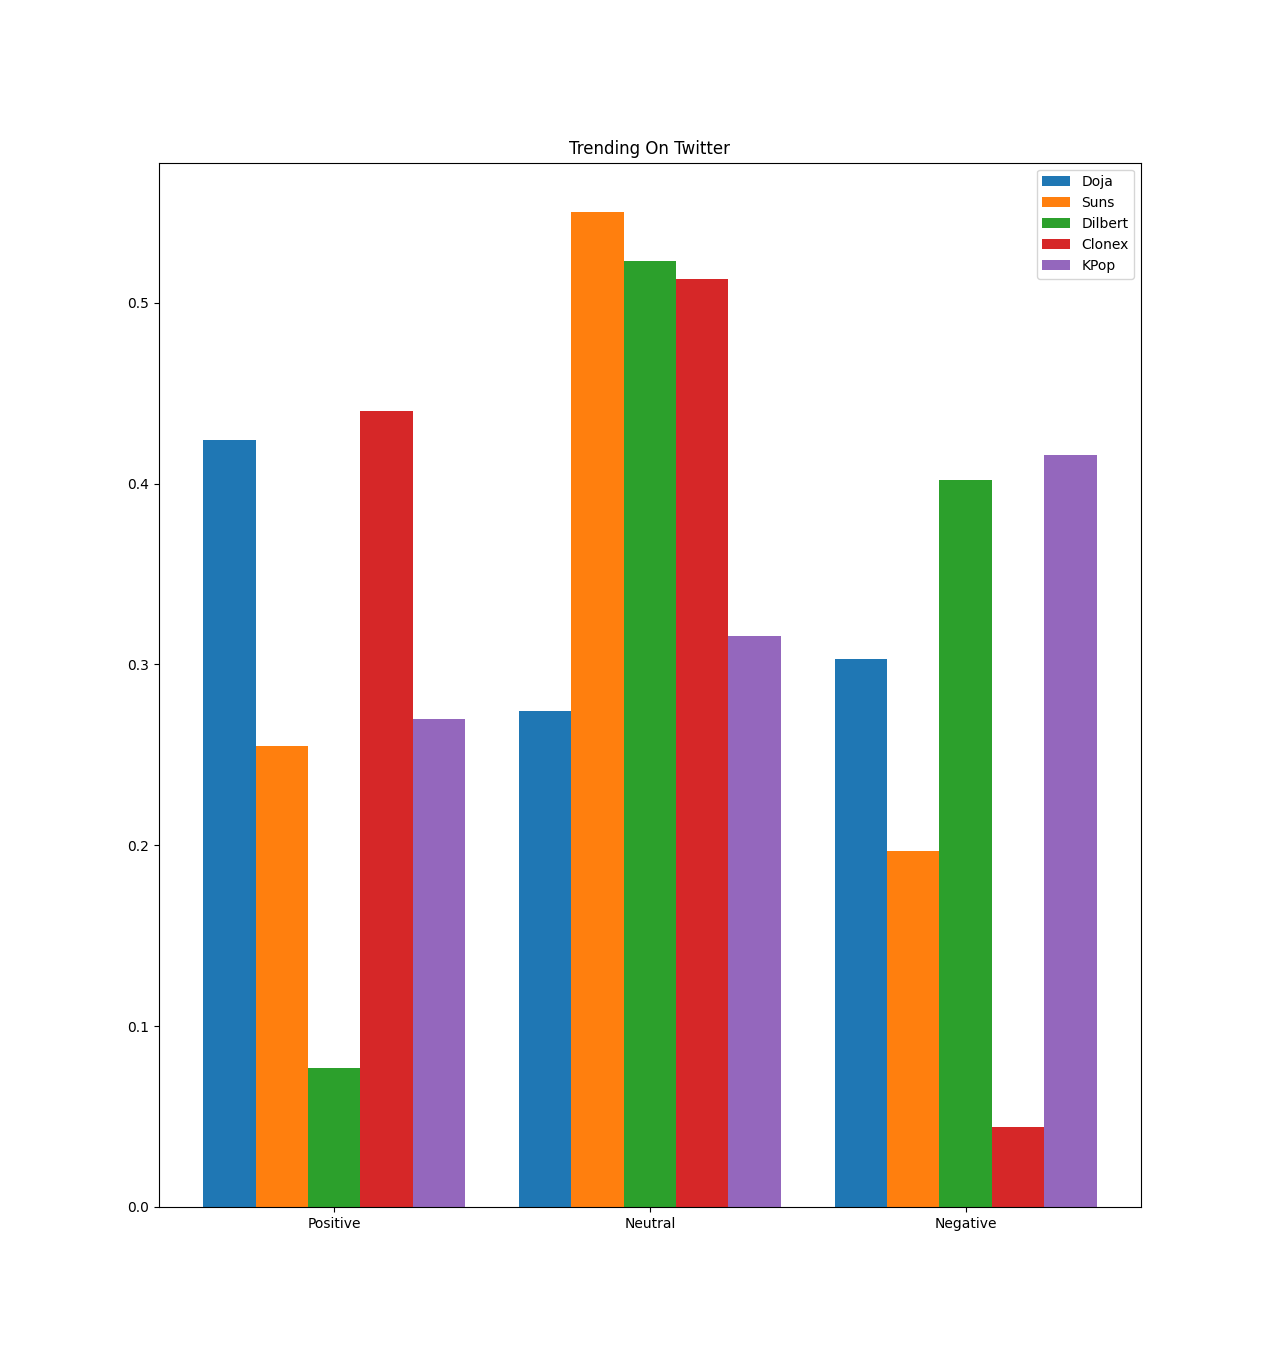
\includegraphics[width=12cm, height=10cm]{trending_on_twitter.png}
        \caption{Twitter Trend Sentiments}
        \label{fig:graph}
    \end{figure}

    The sentiment analysis received from the agent was then averaged and graphed as shown in Figure \ref{fig:graph}.
    Now from the data collected, conclusions can be drawn based off of the analysis. ``Doja'' is positive for the 
    majority, so it is likely the concert went well. ``Suns'' is mostly neutral, but with a larger percentage
    of positivity. This is likely due to a majority of the tweets stating the games score or current game updates, 
    while the positive tweets are likely fans celebrating, and negative tweets are likely fans of the losing team
    expressing their frustration or disappointment. ``Dilbert'' is overwhelmingly more negative than positive. From
    this we can assume that the comments made by the author were indeed unfavorable to the majority of people, and 
    my internet reporter persona would be wise to cash in on the controversy for easy clicks. ``Clonex'' is 
    overwhelmingly positive, which shows that the majority of people are very pleased with the company's performance.
    And finally, ``K-Pop'' is largely divided, with around one-third in each category. This shows that the genre
    of music is rather divisive, with fans loving it and others hating it.

    The results from the two different poems were different that what would be assumed. The happy poem [3] did return
    with an overall positive perception, with the positive category scoring 0.91. The sad poem [4] however, did not
    return a negative sentiment. It, in fact, also returned a positive sentiment, with total positive, neutral and 
    negative ratings of 0.72, 0.22, and 0.06 respectively. Not only did it perceive the poem as positive, but negative
    was the lowest rating it received. Upon further examination, it is likely due to the individual sentences in the
    poem. Lines like ``What is the point of celebrating'', while negative to a human, could be seen as neutral due
    to it simply being a question, or even positive due to the inclusion of the word celebrating, which comes from the 
    word ``celebrate'', a typically positive word. 

    \section{Discussion}
    Obviously, checking twitter and analyzing poems is not the only application for this type of technology. 
    Other applications for this type of data could be a marketing department wanting to know how people are reacting
    to their latest product or commercial; a cellular consumer wanting to know what people think of the newest 
    smart-phone; or a television studio wanting to know how their latest episode was received. The applications
    are practically endless.

    Something I found interesting while working on this, was that, as it stands, the overall sentiment of a text,
    as perceived by a machine, is a collection of individual scores given to sentences. This seems obvious at first,
    but it actually can change the perception of the entire text. Take the example with the sad poem. When read as 
    an entire work, it quite obviously appears sad, and I don't think it too strange to assume that others will agree.
    It takes a very bleak perspective on life, with little hope for the future. Most humans will read this and 
    feel sad or depressed as a result. The agent, however, broke it into its individual words and sentences and 
    interpreted it from there. Words like ``celebrating'' and  ``loved'' likely account for the overall positive 
    sentiment of the poem, while phrases like ``Another year of struggling alone'' and ``The past has left its scars'',
    while seen as negative by humans, would likely be seen as neutral or only mildly negative to an agent.

    \section{Related Works}
    Sentiment analysis, and its related field, opinion mining is one of the major tasks of natural language processing.
    As a result there are various works conducted relating to it. One such work was done in 2015 by Xing Fang and Justin Zhan,
    where they attempted to tackle the problem of sentiment polarity categorization, one of the fundamental problems of 
    sentiment analysis. They did this by using online product reviews from Amazon.com, and conducted experiments for
    both sentence-level categorization and review-level categorization, using multiple different machine learning techniques.
    In the end, they were able to help tackle this issue, by using scikit-learn, an open source machine learning software
    package in python, and selected the models Naive Bayesian, Random Forest, and Support Vector Machine for categorization.[5]

    In an even more related work, in 2016, Kahlil Philander and YunYing Zhong also used sentiment analysis with Twitter data
    to build low-cost and real-time measures of hospitality customer attitudes / perceptions. To do this, they used a popular
    tourist destination (Las Vegas, NV) as the case study. They created a sentiment index for every Twitter account belonging
    to an integrated-resort property in the Las Vegas metropolitan area. From the metrics they received, they were able to 
    benchmark these firms against one another, and compare their performance over time. They concluded that sentiment analysis
    can and does provide an avenue for cheap and real-time feedback on customer service.[6]

    \section{Conclusion}
    In conclusion, natural language processing is an important aspect of artificial intelligence in our daily lives. Sentiment
    analysis in particular has several cheap and real-time applications for businesses and individuals alike. In this paper, 
    I have discussed the process and results of my own experiments, and found them to be successful, even though the results 
    with the sad poem surprised me, and went contrary to what I hypothesized. Were I to repeat the process, I would attempt to 
    gain access to a educational Twitter developer account, allowing for historical data retrieval, and an upgraded Microsoft 
    Cognitive Service account, allowing for more analysis. Other options would be to look for an open-source solution for 
    sentiment analysis, as it is likely there are python packages that contain the resources necessary.

    \section{References}
    [1] Simplilearn. Natural Language Processing In 5 Minutes | What Is NLP And How Does It Work? | Simplilearn (March 17, 2021).
    Accessed: April 12, 2022. [Online Video]. Available: https://www.youtube.com/watch?v=CMrHM8a3hqw\\

    \noindent[2] docs.tweepy.org, 'Tweepy Documentation', 2009. [Online].\\ Available: https://docs.tweepy.org/en/stable/  [Accessed: April 12 2022]\\

    \noindent[3] Sri Aurobindo. "Book II The Book of the Traveller of the Worlds Canto XIV The World-Soul" [Online]. Available: https://www.shortpoems.org/poems/happiness-short-poems/ [Accessed April 17, 2022]\\

    \noindent[4] John P. Read. "No Celebration". February 2017 [Online]. Available: https://www.familyfriendpoems.com/poem/no-celebration [Accessed April 17, 2022]\\

    \noindent[5] Xing Fang and Justin Zhan, "Sentiment analysis using product review data".\textit{The Journal of Big Data}, vol. 2, no. 1, pp. 1-14, June 2015.
    DOI: 10.1186/s40537-015-0015-2\\

    \noindent[6] K. Philander Y. Zhong, `Twitter sentiment analysis: Capturing sentiment from integrated resort tweets', International Journal of Hospitality Management, T. 55,  16-24, 2016.






    

\end{document}